%!TEX root = ../dissertation.tex
%\begin{savequote}[75mm]
%Nulla facilisi. In vel sem. Morbi id urna in diam dignissim feugiat. Proin molestie tortor eu velit. Aliquam erat volutpat. Nullam ultrices, diam tempus vulputate egestas, eros pede varius leo.
%\qauthor{Quoteauthor Lastname}
%\end{savequote}

\chapter{Analisi prestazionale}

\newthought{Per effettuare un'analisi prestazionale} del crittosistema sviluppato, è doveroso tenere conto di diverse variabili. Tra queste spiccano il tempo e lo spazio di memoria necessari per la generazione delle chiavi.

%
%
\section{Generazione di numeri primi}
%
%

Il processo che più di tutti appesantisce la generazione delle chiavi è sicuramente quello che porta alla generazione di un numero primo. Infatti, come approfondito nel capitolo ``Test di primalità'', viene trovato, in media, un numero primo lungo $1kbit$ ogni 355 numeri interi dispari casuali. Questo vuol dire che dovranno essere effettuati altrettanti test più o meno dispendiosi, per determinare la primalità di un numero dispari. 

Le lunghezze interessate per questo tipo di test sono cinque, ovvero:
\begin{itemize}
	\item 128 bit;
	\item 256 bit;
	\item 512 bit;
	\item 1024 bit;
	\item 1536 bit.
\end{itemize}

Le prime tre rappresentano quello che è stato lo standard richiesto negli anni precedenti, la quarta rappresenta lo standard odierno, mentre l'ultima rappresenta lo standard richiesto nel prossimo decennio. Si ricorda che le lunghezze imposte ai numeri primi sono la metà rispetto alla lunghezza della chiave $n$.

I test sono stati effettuati in ambiente Linux, più in particolare su un server Ubuntu equipaggiato di:
\begin{itemize}
	\item n.4 CPU AMD EPYC\ap{TM} 7501, 32 core, 64 threads, con una frequenza base di 2.0GHz;
	\item 8GB di RAM di tipo DDR4.
\end{itemize}

Di seguito viene riportata la tabella contenente i dati registrati durante i test. Sono stati generati, per ogni lunghezza, 100 numeri primi casuali e per ognuno di questi sono stati registrati:
\begin{itemize}
	\item il tempo medio necessario alla generazione di un numero primo;
	\item il numero medio di interi generati prima di trovare un numero primo;
	\item il tempo medio necessario a valutare la primalità di ogni singolo numero intero generato.
\end{itemize}

È interessante aggiungere una quinta colonna alla tabella il tempo impiegato dal calcolatore ad eseguire i test di primalità per ciascun bit. In questo modo si verifica come la lunghezza della chiave incida sulla complessità di calcolo dell'algoritmo.

\begin{table}[h]
	\label{prestazionePrimi}
	\centering
	\begin{tabular}{ccccc}
		\toprule
		Lunghezza & Tempo & \# di interi testati & Tempo per numero & Tempo per bit \\
		($bit$) & ($s$) & (\#) & ($ms / \text{\#}$) & ($ms / \text{\#} \cdot bit$) \\
		\midrule
		128 & 0,063 & 45 & 1,7 & 0,0133 \\
		256 & 0,374 & 87 & 4,9 & 0,0191 \\
		512 & 3,082 & 212 & 16,4 & 0,0320 \\
		1024 & 20,087 & 374 & 58,1 & 0,0567 \\
		1536 & 67,877 & 570 & 122,8 & 0,0799 \\
		\bottomrule
	\end{tabular}
	\caption{Misurazione delle prestazioni per la generazione di numeri primi di lunghezza indicata.}
\end{table}

\begin{figure}
	\centering
	\subcaptionbox{Corrispondenza lunghezza / tempo\label{subfig:tempo}}{
		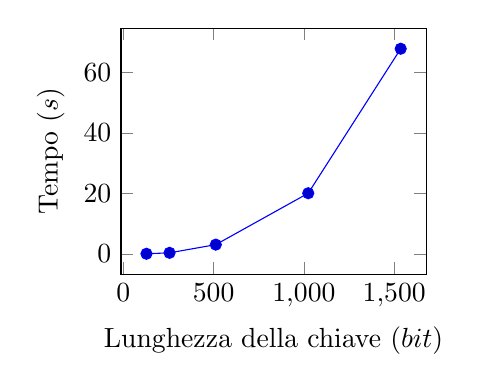
\begin{tikzpicture}
			\begin{axis}[xlabel={Lunghezza della chiave ($bit$)}, ylabel={Tempo ($s$)}, width=.45\textwidth]
				\addplot coordinates {(128, 0.063) (256, 0.374) (512, 3.082) (1024, 20.087) (1536, 67.877)};
			\end{axis}
		\end{tikzpicture}
	}
	\hfill
	\subcaptionbox{Corrispondenza lunghezza / interi testati\label{subfig:interi}}{
		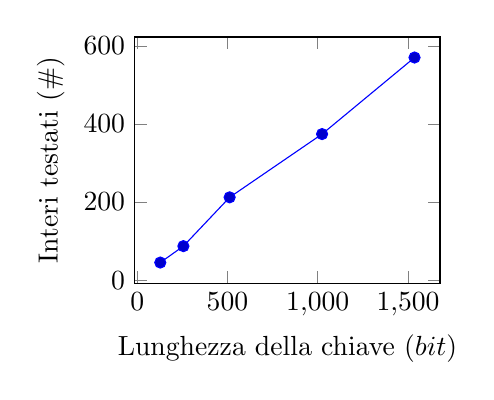
\begin{tikzpicture}
			\begin{axis}[xlabel={Lunghezza della chiave ($bit$)}, ylabel={Interi testati (\#)}, width=.45\textwidth]
				\addplot coordinates {(128, 45) (256, 87) (512, 212) (1024, 374) (1536, 570)};
			\end{axis}
		\end{tikzpicture}
	}
	
	\vspace{1.75em}
	
	\subcaptionbox{Corrispondenza lunghezza / tempo per interi testati\label{subfig:tempointeri}}{
		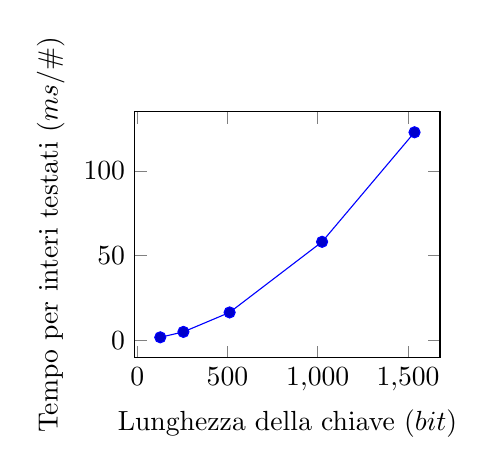
\begin{tikzpicture}
			\begin{axis}[xlabel={Lunghezza della chiave ($bit$)}, ylabel={Tempo per interi testati ($ms / \text{\#}$)}, width=.45\textwidth]
				\addplot coordinates {(128, 1.7) (256, 4.9) (512, 16.4) (1024, 58.1) (1536, 122.8)};
			\end{axis}
		\end{tikzpicture}
	}
	\hfill
	\subcaptionbox{Corrispondenza lunghezza / tempo per bit\label{subfig:tempobit}}{
		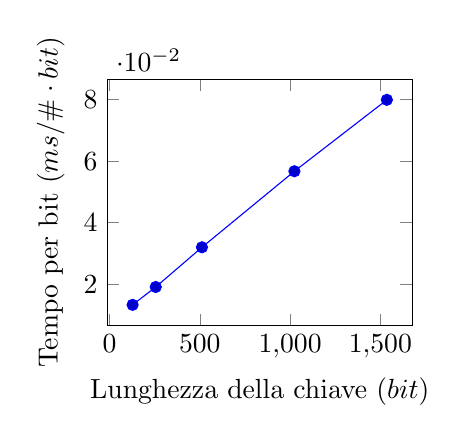
\begin{tikzpicture}
			\begin{axis}[xlabel={Lunghezza della chiave ($bit$)}, ylabel={Tempo per bit ($ms / \text{\#} \cdot bit$)}, width=.45\textwidth]
				\addplot coordinates {(128, 0.0133) (256, 0.0191) (512, 0.0320) (1024, 0.0567) (1536, 0.0799)};
			\end{axis}
		\end{tikzpicture}
	}
	\caption{Prestazione test di primalità.}
	\label{fig:testPrimality}
\end{figure}

Come si evince dai grafici rappresentati nella figura \ref{fig:testPrimality}, il tempo medio necessario a generare un numero primo cresce, con l'aumentare della lunghezza del numero stesso, seguendo un andamento esponenziale. Anche il tempo medio impiegato per testare ogni singolo numero generato prima di trovare un numero primo (fig.~\ref{subfig:tempointeri}) segue un andamento esponenziale, ma la forza con cui la curva sale è minore rispetto al grafico precedente.

La curva che indica il numero di interi generati e testati prima di trovare un numero primo (fig.~\ref{subfig:interi}) e quella che indica il tempo medio necessario ad effettuare il test per ciascun bit generato (fig.~\ref{subfig:tempobit}) seguono, tuttavia, un andamento che può essere definito lineare.

%
%
\section{Generazione della coppia di chiavi}
%
%

La creazione dei numeri primi richiede la quasi totalità del tempo di esecuzione del processo che genera la coppia di chiavi. Nella tabella seguente, si può notare tale occupazione in termini percentuali. Nonostante una lieve retrocessione, la percentuale di tempo dedicato al calcolo dei numeri primi $p$ e $q$ tende a prevalere sul resto, fino a rendere quasi irrilevante il tempo necessario ad effettuare tutti i controlli a generare il resto della coppia di chiavi.

\begin{table}[h]
	\label{tempiGenerazioneChiavi}
	\centering
	\begin{tabular}{ccccc}
		\toprule
		Lunghezza & \splitCell{Tempo\\intero\\processo} & \splitCell{Tempo\\calcolo\\primi} & \splitCell{Tempo\\rimanente} & \splitCell{Occupazione\\calcolo\\primi} \\
		($bit$) & ($s$) & ($s$) & ($s$) & (\%) \\
		\midrule
		256 & 0,1402 & 0,126 & 0,0142 & 90\% \\
		512 & 0,8360 & 0,748 & 0,0880 & 89\% \\
		1024 & 7,0768 & 6,164 & 0,9128 & 87\% \\
		2048 & 40,8828 & 40,174 & 0,7088 & 98\% \\
		3072 & 136,9689 & 135,754 & 1,2149 & 99\% \\
		\bottomrule
	\end{tabular}
	\caption{Misurazione dei tempi medi di generazione delle coppie di chiavi di lunghezza indicata.}
\end{table}


%
%
\section{Spazio di memoria}
%
%

Mantenendo la stessa configurazione del server Ubutnu illustrata in precedenza, si è studiata l'occupazione di memoria dovuta all'implementazione del crittosistema. Il file eseguibile, compilato con il compilatore \emph{GNU Compiler Collection}, occupa $32KB$ della memoria di massa. L'occupazione della memoria RAM, quantificata mentre il processo è in esecuzione, è di circa $4700B$. Per avere una stima più accurata, sarebbe necessario compilare la mappa di memoria.

























































